\documentclass[11pt]{article}

\usepackage[review]{acl}
\setlength{\linenumbersep}{6pt}
\AtBeginDocument{\switchlinenumbers*}
\makeatletter
% TeX Live 2026 lineno can place first-page ACL review numbers in the column
% gutter because of the \twocolumn[\maketitle] title block. Keep the review
% ruler on body pages, but suppress the visually broken first-page numbers.
\let\acl@orig@makeLineNumberLeft\makeLineNumberLeft
\let\acl@orig@makeLineNumberRight\makeLineNumberRight
\renewcommand\makeLineNumberLeft{\ifnum\value{page}=1\relax\else\acl@orig@makeLineNumberLeft\fi}
\renewcommand\makeLineNumberRight{\ifnum\value{page}=1\relax\else\acl@orig@makeLineNumberRight\fi}
\makeatother

\usepackage{times}
\usepackage{latexsym}
\usepackage[T1]{fontenc}
\usepackage[utf8]{inputenc}
\usepackage{microtype}
\usepackage{inconsolata}
\usepackage{graphicx}
\usepackage{booktabs}
\usepackage{multirow}
\usepackage{tabularx}
\usepackage{enumitem}
\usepackage{amsmath}
\usepackage{amssymb}

\newcommand{\task}{evidence-grounded response resolution}
\newcommand{\dataset}{RegTrace-SEC}
\newcommand{\cmsdataset}{RegTrace-CMS}
\newcommand{\framework}{RegTrace-Agent}

\title{\framework{}: A Context-to-Feedback Framework for\\
Evidence-Grounded Regulatory Response Review}

\author{Anonymous ACL submission}

\begin{document}
\maketitle
\begin{abstract}
Financial LLM systems are increasingly asked to judge whether an institution's response actually resolves a prior review request, yet most financial benchmarks still evaluate static QA, extraction, or classification. We introduce \framework{}, a context-to-feedback-review framework for \task{}. Given a reviewer request, an organizational response, and revised or corrective artifacts, the framework retrieves context, decomposes obligations, verifies visible gaps, converts adjudicated failures into scalar/category/natural-language feedback, and trains a reusable reviewer policy. We instantiate the framework primarily on SEC comment-letter review, constructing \dataset{}, 472 public EDGAR examples with amended-filing evidence, visible-evidence labels, feedback fields, and later same-topic SEC follow-up signals. We further test cross-regulatory adaptation on CMS-2567 Plans of Correction and an FDA warning-letter stress test, where the framework must reshape the task because public company responses are not observable. Across SEC grouped, temporal, and topic-holdout settings, full natural-language feedback is the strongest reviewer-training signal among handwritten prompting, MIPROv2, and scalar/category GEPA variants; on CMS, domain-specific full-feedback optimization beats generic and scalar/category controls; on FDA, recursive rubric calibration improves a reshaped warning-to-closeout verifier. Qualitative traces show how feedback turns a terse reviewer into an obligation-evidence policy that can reject unsupported revision claims while avoiding over-requirement when a corrective plan or closeout trace is already materially adequate.
\end{abstract}

\section{Introduction}

Financial NLP has rapidly moved toward LLM systems for long documents, domain-specific reasoning, and decision support. Models and benchmarks such as BloombergGPT, FinGPT, FinBen, FinanceBench, FinQA, TAT-QA, and ConvFinQA show both the promise of financial LLMs and the continuing difficulty of grounding answers in financial evidence \citep{wu2023bloomberggpt,yang2023fingpt,xie2024finben,islam2023financebench,chen2021finqa,zhu2021tatqa,chen2022convfinqa}. Recent FinNLP work has similarly emphasized retrieval-augmented financial QA, SEC filing QA, financial intelligence benchmarks, factuality judging, and evasive-answer detection \citep{lithgow2025rag,lai2025secqa,klimaszewski2025avenibench,wu2025nli,nuaimi2025evasive}. Most such settings, however, still present a static input and ask for a static answer, label, or report.

Many operational finance and compliance workflows have a different structure. A regulator, auditor, lender, or control function requests a correction, explanation, disclosure, or supporting artifact; the organization responds that it has revised an external document; the reviewer must decide whether visible evidence actually satisfies the request. For example, a company may reply that it revised a filing to address a requested forecast disclosure, while the amended filing only shows combined revenue projections and still omits the requested entity-level assumptions. The task is therefore not to judge whether the response sounds cooperative, but whether the repaired artifact visibly closes the original gap. We call this class of problems \task{}. It is related to fact verification and document-level legal NLI \citep{thorne2018fever,koreeda2021contractnli}, but adds a prior reviewer request, a response that may only claim a revision, revised evidence that must be checked, and textual feedback about what remains missing.

Existing work leaves three limitations for this setting. First, benchmarks rarely ask whether an organization has repaired a documented deficiency. Second, response evaluation often has weak obligation grounding: a response can sound persuasive while amended evidence omits a named disclosure, quantification, exhibit, legal basis, or accounting analysis. Third, prompt and pipeline optimization often discards feedback structure by receiving only scalar success, although review failures are naturally described in text: what was requested, what was claimed, what evidence showed, and what gap remained.

We study these limitations through U.S. Securities and Exchange Commission (SEC) comment-letter review. SEC staff issue comments requesting expanded disclosure, clarification, revised accounting discussion, removal of unsupported statements, or additional exhibits; companies respond in writing, often with statements such as ``the disclosure has been revised accordingly.'' After review completion, the SEC releases staff comment letters and company responses through EDGAR. These traces often point to amended filings and sometimes include later same-topic SEC follow-up comments. Accounting research treats comment letters as economically meaningful regulatory signals \citep{cassell2013sec,bozanic2017sec,baugh2023auditor,ryans2021comment}; for NLP, they provide observable request-response-evidence-feedback traces.

We introduce \framework{}, a context-to-feedback-review framework for evidence-grounded reviewers. It reconstructs review traces, retrieves revised or corrective context, decomposes requests into obligations, adjudicates visible gaps, compiles scalar/category/full feedback, and optimizes a guarded reviewer policy. The learned reviewer is not a single hand-tuned prompt; it is the policy inside a system that gathers evidence, checks obligations, emits a guarded verdict, and uses adjudicated failures to improve the next offline reviewer. This framing is deliberately broader than SEC filings: the same loop applies whenever an organization responds to a reviewer by claiming to fix a document, process, artifact, or remediation plan.

This design makes response resolution a strong testbed for language-feedback optimization. Prompt-programming work treats LLM pipelines as declarative programs whose prompts and demonstrations can be optimized \citep{khattab2023dspy}; GEPA argues that natural-language feedback can expose reusable failure structure that scalar reward discards \citep{agrawal2026gepa}. In our setting, that structure is regulator-style: a mistake can be explained as a missing requested disclosure, unsupported revision claim, absent exhibit, or incomplete analysis.

The above limitations motivate three research questions. RQ1 asks whether public review traces can be converted into a benchmark for evidence-grounded response resolution. RQ2 asks whether full natural-language feedback is a stronger reviewer-training signal than scalar prompt search and coarse categories. RQ3 asks whether the resulting decisions generalize across threads, time, and issue categories, and whether unresolved decisions are corroborated by later regulator follow-up.

We make four contributions. First, we define \task{} and introduce \framework{}, a context-to-feedback-review framework for evidence retrieval, obligation checking, feedback construction, adaptive trace specification, and reviewer optimization. Second, we instantiate it as \dataset{}, a public EDGAR benchmark with SEC comments, company responses, amended-filing evidence, labels, and feedback fields. Third, we show that full natural-language feedback is the strongest reviewer-training signal, outperforming handwritten prompting, MIPROv2, scalar/category GEPA variants, and a supervised lexical baseline; a guarded verifier distilled from the learned policy improves further. Fourth, we provide evidence ablations, independent-feedback and feedback-component ablations, prompt-evolution analysis, systematic corroboration from real next-round SEC follow-up comments, and cross-regulatory studies on CMS and FDA showing that the framework transfers as an adaptive construction-and-feedback pattern rather than as a verbatim SEC prompt.

\section{Related Work}

\paragraph{Financial NLP and evidence-grounded evaluation.}
Financial NLP has moved from broad document classification toward long-document reasoning, evidence grounding, and compliance-sensitive decisions. FinQA, TAT-QA, and ConvFinQA introduced financial reasoning questions over reports, tables, and conversations \citep{chen2021finqa,zhu2021tatqa,chen2022convfinqa}; FinanceBench evaluates open-book QA over company documents \citep{islam2023financebench}. Recent FinNLP work has similarly emphasized RAG over financial documents, accessible finance-intelligence benchmarks, factuality and causality judging, SEC filing QA, and evasive-answer detection \citep{lithgow2025rag,klimaszewski2025avenibench,lai2025secqa,nuaimi2025evasive,wu2025nli}. Our task differs by asking whether retrieved evidence satisfies a prior regulator request.

\paragraph{SEC comment letters and regulatory review.}
Accounting and disclosure research has studied SEC comment letters as regulatory signals, including remediation costs, disclosure effects, recurring disclosure deficiencies, and textual classification of comment-letter topics \citep{cassell2013sec,bozanic2017sec,baugh2023auditor,ryans2021comment}. That literature generally treats comment letters as economic or disclosure events. We instead treat the correspondence as document-grounded supervision for LLM systems. Each review unit contains a staff request, company response, amended filing evidence, and sometimes a next-round SEC follow-up.

\paragraph{Prompt optimization and language feedback.}
DSPy reframes LLM pipelines as declarative programs whose prompts and demonstrations can be optimized against metrics \citep{khattab2023dspy}. MIPROv2 and related optimizers primarily use scalar feedback. A broader line studies language feedback, including self-refinement, verbal reinforcement, and critique-based training \citep{scheurer2022language,madaan2023selfrefine,shinn2023reflexion}. GEPA uses natural-language reflection over execution traces \citep{agrawal2026gepa}. This distinction is central here because SEC response errors are naturally textual: missing disclosures, unsupported revision claims, absent exhibits, incomplete analysis, or over-demand beyond the SEC request.

\section{\framework{} Framework}

\subsection{General Review-Trace Setting}

\framework{} applies to workflows where a response claims to satisfy a prior review request by modifying or supplying evidence outside the response itself. Formally, each review trace contains a request $q$, a response $r$, a collection of revised or supporting artifacts $\mathcal{D}$, and optional later reviewer feedback $u^+$. The system retrieves evidence $e=R(q,r,\mathcal{D})$, extracts obligations $o_{1:m}=O(q)$, and applies a verifier $V(q,r,e,o_{1:m})$ whose output is either \texttt{resolved} or \texttt{unresolved}.
The same trace can also produce feedback for learning. A scalar signal says whether the prediction is correct. A category signal names a broad issue or gap type. A full natural-language signal describes the request, the response action, the visible evidence, and any unmet requirement. This makes the framework applicable beyond SEC review whenever request-response-evidence traces are available.

\begin{figure*}[t]
\centering
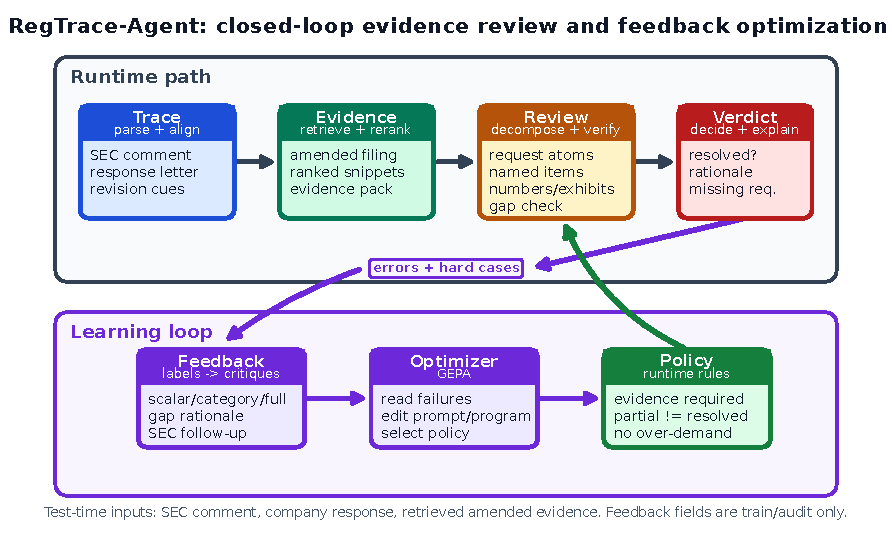
\includegraphics[width=\textwidth]{figures/regtrace_agent_framework.pdf}
\caption{\framework{} architecture. A domain adapter first maps a corpus into request, response, evidence, label, feedback, and optional external-corroboration roles. The runtime path parses a review trace, retrieves or selects evidence, checks obligations, and emits a guarded verdict. The learning loop stores scalar, category, and natural-language feedback, lets GEPA revise the reviewer policy, and reinjects the learned policy into the obligation-review step. At test time the reviewer sees only domain-approved input fields, never adjudication rationales or feedback fields.}
\label{fig:pipeline}
\end{figure*}

\subsection{Adaptive Trace Construction}

The first stage of \framework{} is a trace-construction agent rather than a fixed SEC preprocessor. For a candidate domain $d$, it emits a \textsc{TraceSpec}
\[
S_d=(\phi_d, y_d, f_d, a_d, \rho_d),
\]
where $\phi_d$ maps local fields into request, response, evidence, metadata, and external-corroboration roles; $y_d$ defines the review label; $f_d$ defines scalar, category, and full-text feedback channels; $a_d$ lists fields forbidden at test time; and $\rho_d$ is a utility decision. The utility decision scores role observability, evidence availability, label viability, feedback richness, external corroboration, release viability, and optimization suitability. If any core role is weak, the agent must either reshape the task or reject it instead of forcing the SEC schema.

This matters because regulatory corpora expose different trace structures. In SEC review, the appropriate trace is staff comment, company response, amended-filing snippets, visible-evidence label, and later same-topic follow-up. In CMS-2567, the response and corrective artifact are often the same Plan of Correction, so the task becomes plan adequacy rather than amended-document verification. In a probe over FDA warning letters, public warning and closeout letters are available, but public company response letters are largely absent; the construction decision is therefore to reshape the domain into warning-to-closeout resolution tracing or add contrastive controls before treating it as a benchmark. The framework is thus recursive at the data level: construction decisions create feedback fields, feedback improves the reviewer, and reviewer failures can trigger schema or rubric revision.

\subsection{SEC Instantiation}

Each SEC example contains three test-time fields: \texttt{sec\_comment}, \texttt{company\_response}, and \texttt{retrieved\_snippets} from amended filings. The output is binary. \texttt{resolved} means visible amended evidence covers the material request; \texttt{unresolved} means a named item, quantification, exhibit, document, legal analysis, accounting analysis, or other material requirement remains missing. The label is a visible-evidence judgment, not a legal determination or an inference from absence of later follow-up.

\subsection{SEC Trace Construction}

Figure~\ref{fig:pipeline} separates the runtime reviewer from the feedback-learning loop. In the SEC instantiation, we harvest \texttt{UPLOAD} and \texttt{CORRESP} materials from EDGAR, group staff comments and company responses into review threads, and select cases where the company claims a disclosure was added, revised, removed, or filed elsewhere. We identify amended filing candidates using filing metadata, amendment references, page and section cues, and response text. Candidate filings are drawn from a window of 10 days before to 60 days after the response date, with at most 8 candidate filings per row. A local lexical ranker retrieves top chunks, and an LLM reranker/adjudicator evaluates the top 3 snippets. From 589 revision-claim cases, 588 have candidate filings and snippets; 472 remain after requiring visible evidence that directly or partially addresses the SEC request. We then adjudicate whether visible evidence satisfies the request and construct labels plus feedback fields.

The retrieval component gives the agent evidence to inspect. The adjudication and feedback layer gives it something to learn from: what the reviewer asked for, what the company claimed to do, what the visible evidence supports, and what remains missing. These adjudication fields are not shown as ordinary test-time inputs. They are used for optimization feedback, audits, and analysis.

\subsection{Scale, Categories, and Splits}

\dataset{} contains 472 examples from 109 SEC review threads and 95 companies. The benchmark focuses on difficult revision-claim cases, and the label distribution is operationally realistic: 153 examples are \texttt{resolved}, and 319 are \texttt{unresolved}. Table~\ref{tab:data} summarizes the corpus and split regimes.

\begin{table}[t]
\centering
\small
\begin{tabular}{lr}
\toprule
\textbf{Quantity} & \textbf{Count} \\
\midrule
Examples & 472 \\
SEC review threads & 109 \\
Companies & 95 \\
Resolved / unresolved & 153 / 319 \\
Examples with verified follow-up & 236 \\
\midrule
Issue categories & 7 \\
Visible-evidence gap types & 8 \\
\bottomrule
\end{tabular}
\caption{Benchmark scale. Issue categories include other disclosure issues, risk factors, SPAC disclosure, revenue recognition, crypto, non-GAAP, and cybersecurity.}
\label{tab:data}
\end{table}

The corpus covers seven issue categories and eight visible-evidence gap types; Appendix~\ref{app:data} gives the full distribution. We use grouped, temporal, and topic-holdout regimes. The grouped split holds out entire review threads (229/104/139 train/dev/test). The temporal split trains on 2022--2023 and tests on 2024--2025 (264/64/144). The topic-holdout split tests transfer to held-out issue categories (279/68/125), including crypto and non-GAAP cases absent from training categories.

\subsection{From Labels to Feedback}

A standard benchmark would stop at binary labels. Our construction preserves the textual structure of each decision. For every example, adjudication records the material SEC request, the company action, evidence relevance, supporting evidence or resolution basis, visible unmet requirement, and a short rationale. This lets us compare increasingly rich optimization signals:
\begin{itemize}[leftmargin=*]
    \item scalar: correct or incorrect;
    \item category: correct/incorrect plus coarse issue or gap type;
    \item full: natural-language feedback describing the SEC request, company action, evidence coverage, and unmet requirement.
\end{itemize}
Full feedback can state that the evidence discusses combined revenue projections but fails to disclose entity-level operating costs, product pricing, gross margins, and forecast limitations. This is the reusable decision rule that scalar metrics discard.

\section{Methods}

\subsection{Prediction Setup}

The prediction model receives the SEC comment, company response, and raw retrieved amended-filing snippets. It returns a binary label and a short rationale. Explicit \texttt{resolved} is scored as resolved. \texttt{unresolved}, \texttt{partially\_resolved}, and other insufficient labels are normalized to unresolved. The rationale is required for inspection but not directly rewarded.

\subsection{Optimization Ladder}

We compare reviewer-training signals rather than evidence access. Baseline prompt is a handwritten reviewer instruction. MIPROv2 is scalar prompt optimization. GEPA-scalar uses reflective prompt optimization with correctness-only feedback. GEPA-category adds coarse category feedback. GEPA-full uses full natural-language adjudication feedback. We also include TF-IDF, a frozen sentence-encoder scoring head, a Jev typed decision gate, and an independent-feedback GEPA ablation for reviewer-facing robustness.

All methods receive the same evidence at test time, isolating the optimization signal rather than evidence access. The key comparison is whether natural-language feedback adds value beyond prompt search itself.

\subsection{Implementation Details}

All main prompt-optimization runs use \texttt{openai/gpt-4o-mini} as the frozen prediction model with temperature 0 and 500 output tokens. GEPA uses the same model as the reflection model with temperature 0.7 and 1500 reflection tokens, seed 17, \texttt{max\_metric\_calls}=150, reflection minibatch size 4, Pareto candidate selection, and 4 evaluation threads. MIPROv2 uses the same prediction and prompt models, 8 trials, 4 prompt candidates, and at most 4 labeled and 4 bootstrapped demonstrations. The frozen encoder scorer uses \texttt{all-MiniLM-L6-v2} with a logistic head over request, response, evidence, and request-evidence matching features. The Jev gate uses a \texttt{choice} question over \texttt{resolved}/\texttt{unresolved}. The evidence reranker/adjudicator also uses \texttt{gpt-4o-mini} at temperature 0. Model aliases rather than dated provider snapshots are recorded in the released artifacts.

\subsection{Optimization as Feedback-Conditioned Search}

We view each method as search over a prompt or prompt program $p$. Given an input $x$ and label $y$, the frozen LLM defines $\hat{y}_{p}(x)=f_{\theta}(x;p)$, and optimization seeks a prompt with high validation reward. The methods differ in what they observe after an error. Scalar optimization observes only correctness. Category feedback adds a coarse gap type. Full feedback adds a short critique describing the request, company action, visible evidence, and unmet requirement.

The intuition is information-theoretic. Let $C$ be the latent cause of failure, such as missing quantification or unsupported revision claim. Full feedback should help when it lowers uncertainty about $C$, because the optimizer can propose a more targeted semantic edit. This is not a general guarantee: a noisy or misaligned language channel can hurt. The hypothesis of \framework{} is that review traces are unusually well suited to language feedback because the failure causes are naturally written as reviewer critiques.

\subsection{What the Optimizer Sees}

During optimization, each candidate prompt is evaluated on development examples. When a prediction is incorrect, the metric returns feedback in one of three forms:
\begin{quote}
\small
\texttt{scalar: incorrect}\\
\texttt{category: incorrect; gap\_type=missing\_specific\_disclosure}\\
\texttt{full: incorrect. The SEC requested X. The company claimed Y. The visible evidence shows Z, but does not show required item W.}
\end{quote}
Full feedback summarizes the adjudicated relationship between the SEC request, response, and retrieved evidence for optimization examples only. It does not reveal hidden evidence at test time; any advantage must come from a better learned checklist for visible-evidence review.

\section{Experiments}

\subsection{Evidence Ablation}

We first test whether amended-filing evidence matters. Table~\ref{tab:evidence} evaluates a response-only condition, a raw-evidence condition, and an oracle evidence-summary condition on the grouped held-out test set.

\begin{table}[t]
\centering
\scriptsize
\setlength{\tabcolsep}{3pt}
\begin{tabular}{lrrrr}
\toprule
\textbf{Input} & \textbf{Acc.} & \textbf{Ma-F1} & \textbf{Res-F1} & \textbf{Unres-F1} \\
\midrule
Response only & 0.712 & 0.575 & 0.333 & 0.817 \\
+ raw snippets & 0.784 & 0.748 & 0.651 & 0.844 \\
+ oracle summary & 0.964 & 0.956 & 0.938 & 0.975 \\
\bottomrule
\end{tabular}
\caption{Evidence ablation. Adding raw amended-filing snippets raises macro-F1 by 17.3 points. The oracle summary is an upper bound, not a deployable baseline.}
\label{tab:evidence}
\end{table}

Response-only prompting cannot verify whether a revision claim is supported. Raw snippets nearly double resolved F1, while the oracle summary shows that much of the remaining difficulty is interpreting snippets against a specific request.

\subsection{Main Context-to-Feedback Results}

Table~\ref{tab:leaderboard} reports the main reviewer-training ladder on the frozen grouped split. All methods receive the same test-time context.

\begin{table*}[t]
\centering
\small
\begin{tabular}{lrrrrrr}
\toprule
\textbf{Method} & \textbf{Acc.} & \textbf{Macro-F1} & \textbf{Res-F1} & \textbf{Unres-F1} & \textbf{Unres-P} & \textbf{Unres-R} \\
\midrule
Majority unresolved & 0.691 & 0.409 & 0.000 & 0.817 & 0.691 & 1.000 \\
Baseline prompt & 0.424 & 0.402 & 0.518 & 0.286 & 1.000 & 0.167 \\
MIPROv2 & 0.655 & 0.652 & 0.619 & 0.684 & 0.929 & 0.542 \\
GEPA-scalar & 0.705 & 0.675 & 0.577 & 0.773 & 0.824 & 0.729 \\
GEPA-category & 0.597 & 0.595 & 0.562 & 0.627 & 0.870 & 0.490 \\
GEPA-full & \textbf{0.784} & \textbf{0.756} & \textbf{0.674} & \textbf{0.839} & 0.867 & \textbf{0.812} \\
\bottomrule
\end{tabular}
\caption{Frozen grouped-split leaderboard. GEPA-full gives the best macro-F1 and unresolved F1 under the same raw-evidence test-time context.}
\label{tab:leaderboard}
\end{table*}

The majority baseline has high accuracy because unresolved examples dominate, but zero resolved F1. The handwritten prompt is conservative: it has perfect unresolved precision but misses most gaps. MIPROv2 improves substantially, GEPA-scalar improves recall, and GEPA-category is too coarse in this run. GEPA-full is strongest overall, improving macro-F1 by 10.4 points over MIPROv2 and 8.1 points over GEPA-scalar. This shows that full feedback is not merely adding more text; it trains the reviewer to compare requested obligations against visible evidence.

Table~\ref{tab:robustness} addresses two alternate explanations and one deployment question. A TF-IDF logistic-regression classifier trained on the same raw evidence reaches only 0.523 macro-F1, so lexical supervision does not explain the GEPA-full gain. A frozen sentence encoder with a trained logistic scoring head reaches 0.667 macro-F1 without generation, and a Jev typed decision gate reaches 0.722, showing that \framework{} can support cheap triage scorers, but still trails the full feedback-trained reviewer. On the same grouped held-out test set ($N=139$), the guarded reviewer improves over a monolithic prompt under both \texttt{gpt-4o-mini} and \texttt{gpt-5.4-mini}, suggesting that obligation-evidence structure matters across backbones. To test possible feedback leakage, we regenerate full textual feedback with an independent \texttt{gpt-5.4-mini} writer that sees only test-time fields plus the gold label, not the original adjudication rationales; GEPA with this feedback reaches 0.750 macro-F1, nearly matching the original 0.756.

\begin{table}[t]
\centering
\scriptsize
\setlength{\tabcolsep}{3pt}
\begin{tabular}{llr}
\toprule
\textbf{Check} & \textbf{Condition} & \textbf{Macro-F1} \\
\midrule
Lexical baseline & TF-IDF, response only & 0.523 \\
Lexical baseline & TF-IDF, raw snippets & 0.523 \\
Scoring head & Frozen encoder, raw snippets & 0.667 \\
Decision gate & Jev typed choice, raw snippets & 0.722 \\
Reviewer structure & 4o-mini monolithic / guarded & 0.638 / 0.808 \\
Reviewer structure & 5.4-mini monolithic / guarded & 0.612 / 0.732 \\
Feedback source & GEPA-full, original feedback & 0.756 \\
Feedback source & GEPA-full, independent feedback & 0.750 \\
Diagnostic upper bound & TF-IDF, oracle evidence summary & 0.858 \\
\bottomrule
\end{tabular}
\caption{Robustness checks on the grouped held-out test set unless noted. The raw-snippet TF-IDF baseline shows that lexical supervision does not explain the main result. Frozen encoder and Jev scorers are cheap triage components. Multi-LLM reviewer runs show that guarded obligation-evidence structure improves over monolithic prompting under two backbones. The independent-feedback ablation shows that GEPA-full does not depend on reusing the original adjudication rationales.}
\label{tab:robustness}
\end{table}

We also compute five-fold out-of-fold results over review-thread groups. Mean macro-F1 is 0.698 for GEPA-full, 0.647 for MIPROv2, 0.609 for GEPA-scalar, 0.545 for GEPA-category, and 0.446 for the handwritten baseline. The fold standard deviations are nontrivial (0.151 for GEPA-full and 0.121 for MIPROv2), so we treat the single grouped split as a headline comparison and the out-of-fold analysis as stability evidence rather than as a deterministic margin claim.

\subsection{Why Full Feedback Helps}

The advantage of GEPA-full is not simply risk aversion. Jev reaches very high unresolved recall (0.958) but lower resolved F1 (0.576), making it useful as a triage gate that flags likely unresolved responses. GEPA-full has lower unresolved recall but higher macro-F1, because it better balances skepticism with evidence sufficiency. It learns when a company revision claim is unsupported, but also when visible amended evidence already satisfies the SEC request.

The mechanism is visible in the feedback channel. Scalar feedback says only that a decision was wrong; category feedback names a coarse gap. Full feedback states what the SEC requested, what the company claimed, what the amended evidence showed, and what requirement remained unmet. This gives the optimizer a reusable review trace rather than a bare reward. The resulting prompt evolution shifts from generic caution to obligation-level comparison: identify material SEC request elements, inspect amended evidence for named disclosures, quantification, exhibits, and legal or accounting analysis, and distinguish partial disclosure from resolution.

The trade-off is cost and calibration. GEPA-full requires adjudicated natural-language feedback and offline optimization, so it is not the cheapest runtime gate. It can also become over-skeptical when evidence substantially satisfies a request but does not present the answer in the exact form the prompt expects. We therefore view Jev and frozen encoders as high-throughput first-pass gates, and GEPA-full as the deeper reviewer for difficult or high-impact cases.

\subsection{Reviewer-Structure Ablation}

The optimization ladder tests feedback richness. We also ask whether reviewer structure matters. Table~\ref{tab:guarded} compares a monolithic judgment, an obligation-guided judgment, and a guarded verifier that requires every material obligation to be visibly satisfied, with GEPA-full as the optimized-prompt reference.

\begin{table}[t]
\centering
\scriptsize
\setlength{\tabcolsep}{4pt}
\begin{tabular}{lrrr}
\toprule
\textbf{Reviewer} & \textbf{Macro-F1} & \textbf{Res-F1} & \textbf{Unres-F1} \\
\midrule
Monolithic reviewer & 0.645 & 0.614 & 0.676 \\
Obligation-guided reviewer & 0.619 & 0.613 & 0.624 \\
GEPA-full optimized prompt & 0.756 & 0.674 & 0.839 \\
RegTrace guarded verifier & \textbf{0.801} & \textbf{0.727} & \textbf{0.874} \\
\bottomrule
\end{tabular}
\caption{Reviewer-structure ablation. The guarded verifier is a policy-distillation prototype derived from the obligation-evidence policy exposed by GEPA-full prompt evolution.}
\label{tab:guarded}
\end{table}

Simply listing obligations is not enough; the gain comes from the guard that requires visible support for each material request. We report this as a policy-distillation prototype rather than the primary optimizer comparison, since it adds human-designed structure after prompt-evolution analysis.

\subsection{Feedback Component Ablation}

Table~\ref{tab:feedback} holds test-time input fixed and changes only optimization-time feedback.

\begin{table*}[t]
\centering
\small
\begin{tabular}{lrrrrrr}
\toprule
\textbf{Feedback} & \textbf{Acc.} & \textbf{Macro-F1} & \textbf{Res-F1} & \textbf{Unres-F1} & \textbf{Unres-P} & \textbf{Unres-R} \\
\midrule
Full feedback & 0.784 & \textbf{0.756} & \textbf{0.674} & 0.839 & 0.867 & 0.812 \\
No evidence rationale & 0.712 & 0.682 & 0.583 & 0.780 & 0.826 & 0.740 \\
No unmet requirement & 0.741 & 0.708 & 0.609 & 0.806 & 0.833 & 0.781 \\
Request + action only & 0.784 & 0.724 & 0.595 & \textbf{0.853} & 0.806 & \textbf{0.906} \\
\bottomrule
\end{tabular}
\caption{Feedback component ablation. Request-action feedback induces aggressive unresolved detection, while full feedback gives the best macro-F1 by calibrating skepticism with evidence rationales.}
\label{tab:feedback}
\end{table*}

Request-action-only feedback induces aggressive skepticism and the highest unresolved recall, but sacrifices resolved F1. Full feedback teaches both sides of the boundary: unmet requirements for unresolved cases and supporting evidence for resolved cases.

\subsection{Temporal and Topic Generalization}

Table~\ref{tab:gen} shows that the optimized prompt transfers beyond the grouped split. In the temporal setting, GEPA-full trains/tunes on 2022--2023 and tests on 2024--2025 material. In the topic setting, test examples include crypto and non-GAAP cases absent from training issue categories.

\begin{table*}[t]
\centering
\small
\begin{tabular}{llrrrr}
\toprule
\textbf{Split} & \textbf{Method} & \textbf{Acc.} & \textbf{Macro-F1} & \textbf{Unres-F1} & \textbf{Unres-R} \\
\midrule
\multirow{4}{*}{Time} 
& Baseline & 0.451 & 0.434 & 0.336 & 0.206 \\
& MIPROv2 & 0.521 & 0.519 & 0.489 & 0.340 \\
& GEPA-scalar & 0.653 & 0.650 & 0.679 & 0.546 \\
& GEPA-full & \textbf{0.826} & \textbf{0.791} & \textbf{0.877} & \textbf{0.918} \\
\midrule
\multirow{4}{*}{Topic}
& Baseline & 0.440 & 0.440 & 0.426 & 0.274 \\
& MIPROv2 & 0.576 & 0.565 & 0.635 & 0.484 \\
& GEPA-scalar & 0.528 & 0.524 & 0.569 & 0.411 \\
& GEPA-full & \textbf{0.784} & \textbf{0.734} & \textbf{0.849} & \textbf{0.800} \\
\bottomrule
\end{tabular}
\caption{Temporal and topic-holdout generalization. GEPA-full transfers substantially better than scalar optimization.}
\label{tab:gen}
\end{table*}

The topic-holdout result argues against a curated-topic explanation. Per-topic breakdowns show GEPA-full improves over MIPROv2 on crypto, non-GAAP, revenue recognition, risk factors, and broad other-disclosure cases, with largest gains in revenue recognition and non-GAAP.

\section{Cross-Regulatory Adaptation: CMS-2567}
\label{sec:cms}

We next ask whether \framework{} is only a curated SEC benchmark or whether the same context-to-feedback-review pattern can be instantiated in a different regulatory domain. We use CMS-2567 nursing-home Statements of Deficiencies and Plans of Correction. The object of review is different from SEC filings: a facility receives a deficiency narrative, submits a Plan of Correction (POC), and the reviewer asks whether the plan materially addresses resident-specific correction, affected population, systemic prevention, monitoring, timing, and accountability. The test-time input is \texttt{deficiency\_text}, \texttt{plan\_of\_correction\_text}, \texttt{ftag}, and \texttt{scope\_severity}. Feedback-only fields record covered elements, missing or weak elements, and a reviewer rationale; correction-outcome metadata is hidden and not used as a gold label because most cases eventually become corrected.

This experiment is intentionally framed as adaptation, not direct zero-shot transfer. The SEC optimized prompt checks amended disclosure against named SEC requests. CMS POC review requires a different calibration: a plan can be adequate without proving that every future monitoring step has already succeeded, but it is not adequate if it merely lists education and audits while omitting a cited resident-specific or systemic deficiency.

We construct a 500-example CMS pilot benchmark with grouped train/dev/test splits by source document (270/90/140 examples). Labels map \texttt{adequate} to \texttt{adequate} and both \texttt{partial} and \texttt{inadequate} to \texttt{not\_adequate}. The grouped test set contains 37 adequate and 103 not-adequate examples. These labels are LLM-adjudicated and therefore weaker than the SEC benchmark; we use the study to test framework portability rather than to claim a fully validated second benchmark.

\begin{table*}[t]
\centering
\small
\begin{tabular}{lllrrrr}
\toprule
\textbf{Method} & \textbf{Seed} & \textbf{Feedback} & \textbf{Acc.} & \textbf{Macro-F1} & \textbf{Adeq-F1} & \textbf{Not-Adeq-F1} \\
\midrule
Direct generic prompt & generic & none & 0.707 & 0.694 & 0.631 & 0.757 \\
Minimal seed & minimal & none & 0.650 & 0.642 & 0.588 & 0.696 \\
GEPA-scalar & minimal & correctness only & 0.671 & 0.663 & 0.610 & 0.716 \\
GEPA-category & minimal & coarse category & 0.643 & 0.635 & 0.583 & 0.688 \\
GEPA-full & minimal & written POC feedback & \textbf{0.743} & \textbf{0.723} & \textbf{0.647} & \textbf{0.798} \\
\midrule
Structured SEC seed & SEC-style & none & 0.736 & 0.449 & 0.051 & 0.847 \\
Structured GEPA-full & SEC-style & written POC feedback & 0.771 & 0.584 & 0.304 & 0.863 \\
\bottomrule
\end{tabular}
\caption{CMS-2567 adaptation on the grouped 140-example test set. The SEC-style checklist does not transfer verbatim: it predicts almost everything as not adequate. Starting from a lightweight CMS reviewer, full written feedback beats scalar/category feedback and a direct generic prompt.}
\label{tab:cms}
\end{table*}

Table~\ref{tab:cms} shows the central pattern. A direct generic CMS prompt is already strong (0.694 macro-F1), which means POC adequacy is closer to ordinary regulatory reading than SEC amended-evidence verification. The SEC-style structured reviewer, however, is too conservative: it predicts only two adequate cases and reaches 0.449 macro-F1 despite high nominal accuracy from class imbalance. This is a useful negative result. \framework{} does not mean transferring a frozen SEC checklist. It means re-instantiating the same loop with domain-appropriate feedback.

Under that adaptation, GEPA-full improves the minimal CMS seed from 0.642 to 0.723 macro-F1, beats scalar feedback by 5.9 points, and beats the direct generic prompt by 2.9 points. The gain is not pure skepticism. GEPA-full predicts fewer adequate cases than the generic prompt, but it also preserves high adequate recall while improving not-adequate F1. The full feedback teaches the reviewer when standard POC language is enough and when it is boilerplate that does not address the cited deficiency.

\paragraph{What transfers.}
The reusable part is not a prompt string. It is the context-to-feedback mechanism: identify the reviewer request or deficiency, map the response to material obligations, use adjudicated text to expose covered and missing elements, and optimize a reviewer around that feedback. SEC review learns ``do not accept a revision claim unless amended evidence contains the named disclosure.'' CMS review learns ``substantial adequacy is enough when the plan covers immediate correction, affected population, systemic prevention, monitoring, and timing, but generic education/audit language is not enough when a cited deficiency component is omitted.''

\section{Third-Domain Stress Test: FDA Warning Letters}
\label{sec:fda}

The CMS study tests positive adaptation. We also test whether the construction layer can avoid a bad adaptation. FDA warning-letter data provides public warning letters and closeout letters, but public company response letters are almost absent in our snapshot. A fixed SEC-style framework would force this into a request-response-evidence task and produce a weak benchmark. \framework{} instead emits a \textsc{TraceSpec} decision of \texttt{reshape-before-benchmark}: the observable task is warning-to-closeout trace verification, not response adequacy.

We construct a minimal FDA contrastive benchmark from 400 linked warning-closeout pairs. Each warning receives one positive candidate, its true linked closeout letter, and one hard negative closeout letter, preferably sampled from the same product and subject. This yields 800 examples with grouped train/dev/test splits by warning URL (480/160/160). The held-out test set is balanced, and 357 of 400 negatives in the full benchmark are same-product and same-subject wrong closeouts.

\begin{table}[t]
\centering
\scriptsize
\setlength{\tabcolsep}{2.5pt}
\begin{tabular}{lrrrr}
\toprule
\textbf{Reviewer} & \textbf{Acc.} & \textbf{Ma-F1} & \textbf{Mat. F1} & \textbf{Wrong F1} \\
\midrule
Generic & 0.919 & 0.918 & 0.912 & 0.925 \\
RegTrace strict & 0.881 & 0.880 & 0.865 & 0.894 \\
RegTrace calibrated & \textbf{0.950} & \textbf{0.950} & \textbf{0.947} & \textbf{0.952} \\
\bottomrule
\end{tabular}
\caption{FDA warning-to-closeout trace verification on a 160-example held-out test set using \texttt{gpt-4o-mini}. The strict RegTrace reviewer catches all wrong closeouts but over-rejects true closeouts. A domain-calibrated reviewer preserves mismatch detection while recovering true matches.}
\label{tab:fda}
\end{table}

Table~\ref{tab:fda} shows the recursive behavior we want from the framework. The first strict reviewer is too skeptical: it catches every mismatched closeout but rejects 19 true matches, often because FDA closeout letters are short and do not repeat every violation. The calibrated reviewer changes the rubric, not the hidden data. It treats firm identity, CMS/reference number, warning date, product or violation family, issuing office, and explicit corrective-action evaluation as the trace criteria, while not requiring the closeout to restate the full warning letter. This improves macro-F1 from 0.880 to 0.950 and also exceeds the generic prompt. FDA therefore serves as a compact third-domain demonstration of adaptive construction: when a corpus lacks a response channel, \framework{} reshapes the task and then calibrates the reviewer to the new document genre.

\section{External SEC Follow-Up Corroboration}

Visible-evidence labels come from an adjudication pipeline, so we test whether they align with later regulator behavior. Verified same-topic next-round SEC follow-up is not the primary label, but it is a useful corroboration signal because it can restate or narrow an unresolved gap.

We additionally audit all 472 examples with an independent \texttt{gpt-5.4-mini} auditor that receives only the SEC comment, company response, and raw retrieved evidence snippets, not the benchmark label, feedback fields, evidence summaries, missing-requirement notes, or later SEC follow-up. The audit agrees with the benchmark label in 345 of 472 cases, reaching 0.731 agreement accuracy and 0.715 macro-F1. We report this as an audit of visible-evidence label consistency, not as expert legal/accounting validation.

\begin{table}[t]
\centering
\scriptsize
\setlength{\tabcolsep}{2pt}
\begin{tabular}{lrrr}
\toprule
\textbf{Group} & \textbf{N} & \textbf{D/P} & \textbf{Rate} \\
\midrule
Unres. + f/u & 160 & 109 & 68.1\% \\
Res. + f/u & 76 & 7 & 9.2\% \\
\bottomrule
\end{tabular}
\caption{Real follow-up corroboration. Later same-topic SEC comments directly or partially corroborate unresolved visible-evidence labels far more often than resolved labels.}
\label{tab:followup}
\end{table}

Among 236 examples with verified follow-up, unresolved cases are corroborated at 68.1\%, while resolved cases are corroborated at only 9.2\% (Table~\ref{tab:followup}). Follow-up availability itself is balanced across labels (49.7\% for resolved and 50.2\% for unresolved; Fisher exact $p=1.0$), so this is not merely an availability artifact.

Following reviewer-style paired analysis, we also treat later follow-up as a noisy external reference on a clean 220-example subset. The benchmark label reaches 0.756 macro-F1 against this signal, compared with 0.590 for five-fold out-of-fold GEPA-full predictions and 0.460 for the handwritten baseline. We therefore use follow-up primarily as label-validity evidence, not as proof that every GEPA-full win is separately corroborated beyond the unresolved base rate.

In one expense-disclosure case, the SEC asked for material components and trend discussion. The company claimed a revision, but retrieved evidence showed only a line item and totals; GEPA-full predicted \texttt{unresolved}, and the next-round SEC follow-up again requested the component breakout. SPAC transaction-background cases show the same pattern for missing negotiation details.

\section{Prompt Evolution and Case Studies}
\label{sec:cases}

\subsection{From Terse Prompt to Reviewer Policy}

Prompt evolution is the most visible evidence that \framework{} is not simply tuning a label instruction. In both domains, the seed prompt is deliberately weak. SEC starts from: ``Classify whether a company resolved an SEC comment using the visible evidence.'' CMS starts from: ``Classify whether a CMS Plan of Correction adequately resolves the deficiency.'' Full feedback then rewrites these seeds into different reviewer policies because the feedback describes different kinds of gaps.

\begin{table*}[t]
\centering
\small
\setlength{\tabcolsep}{4pt}
\begin{tabular}{p{0.17\textwidth}p{0.33\textwidth}p{0.42\textwidth}}
\toprule
\textbf{Policy} & \textbf{What the prompt learns} & \textbf{Representative optimized language} \\
\midrule
SEC seed & Generic evidence check. & ``Classify whether a company resolved an SEC comment using the visible evidence.'' \\
\midrule
SEC GEPA-full & Compare named SEC requests against amended evidence; distrust unsupported revision claims; find missing disclosures, quantification, exhibits, and legal/accounting analysis. & ``Carefully compare the SEC request against the company's response and the amended evidence'' and look for ``specific items,'' ``quantification,'' ``detailed analysis,'' and ``visible unmet requirements.'' \\
\midrule
CMS seed & Generic POC adequacy check. & ``Classify whether a CMS Plan of Correction adequately resolves the deficiency.'' \\
\midrule
CMS GEPA-full & Judge substantial POC adequacy: resident-specific correction, affected population, systemic prevention, staff education, monitoring, timing, accountability, and material omissions tied to the deficiency narrative. & Assess whether the POC provides ``clear, actionable steps,'' ``resident-specific corrections, systemic changes, staff education, and ongoing monitoring,'' and avoid relying on ``vague or boilerplate language.'' \\
\bottomrule
\end{tabular}
\caption{Prompt evolution under full feedback. The SEC and CMS optimized prompts share the same context-to-feedback mechanism, but they learn different domain policies. SEC focuses on visible amended disclosure; CMS focuses on whether a remediation plan materially covers the deficiency.}
\label{tab:prompt_compare}
\end{table*}

The component analysis in Table~\ref{tab:prompt} shows the same pattern quantitatively. Scalar and category feedback learn generic caution: company claims need support. Full feedback more consistently induces named-request matching and missing-item reasoning, shifting the policy from generic skepticism to obligation-level comparison: request $\rightarrow$ response action $\rightarrow$ visible evidence or correction plan $\rightarrow$ remaining gap.

\begin{table}[t]
\centering
\scriptsize
\setlength{\tabcolsep}{3pt}
\begin{tabular}{lrrrr}
\toprule
\textbf{Method} & \textbf{Claim} & \textbf{Evidence} & \textbf{Request} & \textbf{Missing} \\
 & \textbf{insuff.} & \textbf{required} & \textbf{match} & \textbf{items} \\
\midrule
GEPA-full & 2/2 & 2/2 & 2/2 & 2/2 \\
GEPA-scalar & 2/2 & 2/2 & 0/2 & 0/2 \\
GEPA-category & 2/2 & 2/2 & 0/2 & 0/2 \\
Req.+action only & 2/2 & 2/2 & 2/2 & 2/2 \\
\bottomrule
\end{tabular}
\caption{Rule presence in SEC optimized prompt candidates. Full feedback more consistently induces named-request matching and missing-item reasoning.}
\label{tab:prompt}
\end{table}

\subsection{What the Feedback Looks Like}

The feedback channel is not a hidden test-time input. It is an optimization-time critique. A SEC unresolved example can return: the SEC requested individual-company forecasts and material assumptions; the company claimed to revise the forecast section; the amended evidence shows combined revenue projections; operating costs, pricing, margins, and forecast limitations remain missing. A CMS not-adequate example can return: the plan covers refrigerator temperature logs but does not address the same deficiency narrative's fall-risk care-plan failure or RN coverage/PBJ issue. These critiques are exactly the information a scalar reward loses.

\subsection{SEC Case: Combined Forecasts Are Not Entity-Level Assumptions}

One SEC comment asked whether the board received VSee and iDoc projections on an individual-company basis and requested entity-level assumptions, including growth rates, operating costs, product pricing, gross margins, and forecast limitations. The company responded that it revised the prospective-financial-information section. The retrieved amended evidence gave combined revenues for 2022 and 2023 and some context about who prepared the projections. The baseline, GEPA-scalar, and GEPA-category predicted \texttt{resolved}; GEPA-full predicted \texttt{unresolved}.

The GEPA-full rationale is qualitatively different. It does not stop at seeing a revised forecast paragraph. It maps the SEC request to named missing requirements: individual-company basis, material assumptions, operating costs, pricing, gross margins, and limitations. This is the regulator-style reasoning we want the system to learn: a response can be responsive in topic but unresolved in obligation coverage.

\subsection{SEC Case: Stablecoin Definition Without the Requested Contrast}

In a crypto disclosure case, the SEC asked the company to clarify what it meant by ``stable cryptocurrency'' as opposed to an ``unstable'' cryptocurrency. The company said it changed the term to ``stablecoin'' and described stablecoins as fiat-pegged assets. The amended evidence defined stablecoins and mentioned examples such as USDC and USDT. Baseline, MIPROv2, scalar GEPA, and category GEPA predicted \texttt{resolved}; GEPA-full predicted \texttt{unresolved}.

The learned policy catches a subtle gap: the evidence defines the stable side but does not directly provide the requested contrast with unstable cryptocurrency. This is not a lexical trick; it is request matching. The optimized SEC prompt tells the reviewer to identify ``specific items or information requested by the SEC'' and verify that amended evidence covers ``all requested aspects.''

\subsection{CMS Case: Full Feedback Is Not Just More Skeptical}

CMS also shows why full feedback is not merely an unresolved detector. In one F0689 resident-safety case, the deficiency was an unsecured treatment cart. The POC gave an immediate teachable moment, identified all residents as potentially affected, trained nursing staff on locked cart storage, reviewed cart storage capacity, and created weekly/monthly accident-hazard audits with QAPI review. The generic prompt predicted \texttt{not\_adequate}, arguing that the plan lacked a direct assurance that carts would always be secured. GEPA-full predicted \texttt{adequate}.

The full feedback for similar adequate cases teaches calibration: substantial adequacy is enough when the plan covers immediate correction, affected population, systemic prevention, monitoring, and timing. This is the opposite of the SEC-style over-skeptical checklist. It shows that full feedback can also reduce false positives by teaching the reviewer not to demand more than the regulatory object requires.

\subsection{CMS Case: Boilerplate Audits Do Not Cover a Multi-Part Deficiency}

In another F0689 case, the deficiency narrative combined several issues: fall-risk care planning for a resident, RN eight-hour coverage/PBJ reporting, and refrigerator temperature monitoring. The POC addressed refrigerator gauges, logs, policy education, and audits. GEPA-scalar and GEPA-category predicted \texttt{adequate}. GEPA-full predicted \texttt{not\_adequate}, because the POC did not visibly correct the fall-risk care-plan problem or the RN coverage/PBJ problem.

This case is the CMS analogue of the SEC projection example. The response contains plausible compliance language and a real corrective action, but only for one component of the deficiency. Full feedback teaches the model to decompose the deficiency narrative and ask whether each material component has a corresponding corrective action.

\subsection{Known Failure Mode}

The same mechanism can over-require. In a SEC ownership-percentage case, retrieved evidence contained redemption-scenario calculations and the benchmark label was \texttt{resolved}. GEPA-full predicted \texttt{unresolved} because it wanted a more explicit cover-page presentation. In CMS, the analogous risk is treating a practical POC as incomplete because it lacks idealized audit escalation language. This is why the guarded verifier and CMS adaptation results should be framed as review-assistant policies with calibrated feedback, not as legal or clinical ground truth.

\section{Discussion}

The main result is not simply that one optimizer beats another. \framework{} turns a recurring compliance pattern into an offline feedback-learning system: collect the trace, retrieve the revised artifact, check obligations against visible evidence, issue a guarded verdict, and recycle adjudicated failures as feedback. The learned reviewer can be used directly, distilled into a guarded verifier, or converted into lightweight scoring heads for high-throughput triage. The output is a traceable unresolved-gap rationale, not only a binary label.

Language feedback helps because it preserves decision structure. A scalar signal says only that a verdict failed; full feedback says which named request, company action, amended snippet, and remaining obligation were mismatched. The optimized prompt therefore becomes an interpretable policy: extract material requests, distrust unsupported revision claims, inspect evidence for named items, avoid over-requiring, and distinguish partial disclosure from resolution.

SEC correspondence is the public setting where we can observe request, response, revised filing, and later reviewer behavior, but the trace structure is broader. Audit remediation, regulatory reporting, lending-document stipulations, data-quality exceptions, and internal compliance monitoring also contain request-response-evidence loops. The transferable claim is that such traces can support retrieval, obligation checking, adjudication feedback, optimized reviewing, and hard-case mining; the limitation is that high-recall language-feedback policies can become over-skeptical.

\section{Conclusion}

We introduced \framework{}, a context-to-feedback framework for evidence-grounded response review, and instantiated it as \dataset{} using public SEC traces. Across grouped, temporal, and topic-holdout evaluations, full natural-language feedback yields the strongest reviewer. Evidence ablations, prompt evolution, and SEC follow-up corroboration suggest that financial NLP benchmarks can move from static labels toward feedback-rich review systems that preserve the reasons behind expert decisions.

\section*{Limitations and Data Statement}

This study is conditioned on visible retrieved evidence, so missed snippets can affect labels. The SEC benchmark is LLM-adjudicated, with independent audit and external follow-up corroboration but without a full expert legal/accounting audit. A full independent \texttt{gpt-5.4-mini} audit over all 472 examples, using only test-time fields, reaches 0.731 agreement accuracy and 0.715 macro-F1 against the released labels. Same-topic SEC follow-up is a noisy behavioral signal, not ground truth. We frame labels as visible-evidence judgments rather than legal determinations. The CMS-2567 study is weaker and should be read as a cross-regulatory adaptation pilot: its 500 labels are primary LLM adjudications, and the \texttt{partial} boundary is noisier than the SEC visible-evidence label. An anonymized release will be provided at \url{https://anonymous.4open.science/r/regtrace-sec-XXXX/}; it includes benchmark JSONL, splits, accession identifiers, retrieval metadata, snippets, labels, feedback fields, prompts, outputs, and analysis scripts.

\clearpage
\bibliography{references}

\appendix

\section{Full Optimized Prompts}
\label{app:prompts}

The main paper quotes short excerpts from optimized prompts. Below are the full GEPA-full optimized candidates exposed by the final grouped-split run. The seed prompt was: ``Classify whether a company resolved an SEC comment using the visible evidence.''

\subsection{GEPA-full Optimized Candidate 1}

\begin{quote}\small
You are tasked with classifying whether a company has resolved a comment from the SEC based on the provided evidence. Follow these instructions carefully:

1. Input Format: You will receive three types of inputs: \texttt{sec\_comment}, \texttt{company\_response}, and \texttt{amended\_evidence}.

2. Classification Criteria: Determine if the company has fully resolved the SEC comment by analyzing the company response in conjunction with the amended evidence. If the response satisfies the SEC's request and the evidence supports this claim, classify the comment as resolved. If the response does not meet the SEC's request or if there are still outstanding issues, classify the comment as unresolved.

3. Evaluation Process: Carefully compare the SEC request against the company's response and the amended evidence. Look for specific items or information requested by the SEC, quantification or detailed analysis that meets SEC requirements, references to regulatory guidance or previous decisions, and clear explanations of how the company adjusted disclosures or practices. Take note of visible unmet requirements, partial fixes, or lack of supporting documentation in the amended evidence.

4. Output Format: Include a reasoning section, a label indicating resolved or unresolved, and a concise reason.

5. Feedback Incorporation: Be vigilant about claims made by the company; ensure that amended evidence corroborates these claims. Identify instances where the response may partially address SEC concerns but still falls short of complete compliance.
\end{quote}

\subsection{GEPA-full Optimized Candidate 2}

\begin{quote}\small
You are tasked with classifying whether a company has resolved a comment issued by the SEC based on provided evidence. Follow these specific instructions for the task:

1. Input Format: You will receive \texttt{sec\_comment}, \texttt{company\_response}, and \texttt{amended\_evidence}. The SEC comment is the original request for clarification or additional information. The company response indicates what changes were made or explanations provided. The amended evidence contains snippets from the amended filing or other documents that support the response.

2. Classification Criteria: Determine whether the company's response and amended evidence adequately address the SEC's concerns as outlined in the original comment. A response is resolved if it fully satisfies the requirements of the SEC comment, including clear explanations, specific details, and quantifications when necessary. A response is unresolved if there are still gaps or missing elements in the company's explanation or if amended evidence does not address all parts of the SEC comment.

3. Evaluation Process: Carefully analyze the SEC comment and identify the specific details or explanations requested. Review the company response to see if the company acknowledged the comment and provided a meaningful response. Examine amended-evidence snippets to confirm that they support the company's claims and cover all requested aspects of the SEC comment. Look for direct references in the amended evidence that address the SEC's specific requests, such as ownership structures, accounting adjustments, or enforcement risks.

4. Labeling: If the company has fully addressed the SEC's concerns with adequate evidence, label the response resolved. If there are omissions or inadequacies in addressing SEC requests, label it unresolved.

5. Justification: Provide clear and concise reasoning that cites specific elements from the SEC comment, company response, and amended evidence. Highlight specific unmet requirements or gaps in the evidence that contribute to an unresolved classification.

6. Feedback Incorporation: Pay attention to feedback from previous examples to identify common pitfalls, such as failing to compare the SEC request against the evidence adequately or missing key elements in the response.
\end{quote}

\section{CMS Optimized Prompt}
\label{app:cms_prompt}

The CMS seed prompt was: ``Classify whether a CMS Plan of Correction adequately resolves the deficiency.'' The full-feedback CMS run under the 270/90/140 grouped split produced a learned reviewer behavior whose outputs emphasize resident-specific correction, systemic prevention, education, monitoring, timing, and material omissions. We report the final reviewer instruction used for the CMS full-feedback policy below. Unlike the SEC appendix above, this is a paper-facing distilled instruction for the optimized CMS reviewer rather than a raw two-candidate state dump.

\begin{quote}\small
Classify the adequacy of a CMS Plan of Correction in resolving identified deficiencies in long-term care facilities. Your evaluation should be based on the specific details of the deficiency and the corresponding Plan of Correction provided. Follow these guidelines:

1. Input Structure: You will receive text inputs including \texttt{deficiency\_text}, a detailed narrative describing the observed deficiency, including specific incidents and regulatory references; \texttt{plan\_of\_correction\_text}, the facility's proposed corrective actions to address the deficiency; \texttt{ftag}, the specific regulatory tag associated with the deficiency; and \texttt{scope\_severity}, the severity and scope level of the deficiency, indicating its impact on residents.

2. Evaluation Criteria: Assess whether the Plan of Correction provides clear, actionable steps to correct the deficiency. Determine if the Plan includes specific actions addressing resident-specific corrections, systemic changes, staff education, and ongoing monitoring. Identify if the Plan outlines a timeline for implementation and a mechanism for quality assurance or follow-up. Look for any vague or boilerplate language that may undermine the effectiveness of the Plan.

3. Response Types: Classify the Plan of Correction as adequate if it sufficiently addresses the identified deficiencies with clear, actionable solutions and monitoring mechanisms; not adequate if it fails to address the core issues outlined in the deficiency, lacks specificity, or does not include necessary follow-up actions; and partial if it includes some corrective actions but lacks comprehensive strategies or fails to address major components of the deficiency.

4. Justification: Provide a clear and concise rationale for your classification, referencing specific elements from both the deficiency text and the Plan of Correction. Highlight any strengths and weaknesses in the Plan based on the criteria outlined above.

5. Feedback Utilization: Incorporate feedback from previous evaluations to refine your assessment process, ensuring that you identify material omissions and weaknesses tied directly to the deficiency narrative rather than relying solely on generalizable strategies.
\end{quote}

\section{LLM-Assisted TraceSpec Constructor Outputs}
\label{app:constructor}

The adaptive construction module asks an LLM constructor to propose a domain-specific \textsc{TraceSpec} from a few examples, then passes the proposal through the executable utility gate. Below are the complete substantive outputs for the three domains. Full JSON artifacts, including token metadata, are released with the code under \url{outputs/adaptive_trace_framework/llm_schema_proposals/}.

\subsection{SEC Constructor Output}

\begin{quote}\small
\textbf{Domain:} sec. \\
\textbf{Task name:} visible-evidence response-resolution review. \\
\textbf{Decision:} \texttt{go-primary-benchmark}. \\
\textbf{Role mapping:} request=\texttt{sec\_comment}; response=\texttt{company\_response}; evidence=\texttt{retrieved\_snippets}, \texttt{amended\_evidence\_best\_snippet}; label=\texttt{visible\_evidence\_resolution\_label}; feedback=\texttt{scalar\_feedback}, \texttt{category\_feedback}, \texttt{full\_feedback}, \texttt{feedback\_sec\_request}, \texttt{feedback\_company\_action}, \texttt{feedback\_evidence\_summary}, \texttt{feedback\_unmet\_requirement}; external corroboration=\texttt{real\_followup\_text}, \texttt{has\_real\_followup}; metadata=\texttt{review\_thread\_id}, \texttt{cik}, \texttt{review\_file\_no}, \texttt{issue\_category}, \texttt{response\_year}. \\
\textbf{Label policy:} resolved iff the visible amended-filing evidence substantially satisfies the material SEC request; unresolved iff a material requested item, quantification, exhibit, document, legal/accounting analysis, or other obligation is still missing from the visible evidence. \\
\textbf{Feedback policy:} scalar=binary correctness against the visible-evidence label; category=issue category plus coarse gap/category feedback; full text=natural-language feedback describing the SEC request, company action, visible evidence coverage, and unmet requirement; external text=later same-topic SEC follow-up text, used only as noisy corroboration. Forbidden at test time: feedback fields, \texttt{full\_feedback}, amended-evidence adjudication fields, and \texttt{real\_followup\_text}. \\
\textbf{Utility scores:} role observability 5.0; evidence availability 4.5; label viability 4.0; feedback richness 5.0; external corroboration 4.0; release viability 4.5; optimization suitability 5.0; mean 4.571. \\
\textbf{Risks:} visible-evidence labels are not expert legal/accounting review; retrieval-conditioned labels can be affected by missing amended-filing evidence. \\
\textbf{Minimal experiment:} review a small subset to validate role mapping and feedback richness. \\
\textbf{Paper claim:} the role mapping and feedback policy align with SEC review because company responses can be evaluated against visible amended-filing evidence and later follow-up.
\end{quote}

\subsection{CMS Constructor Output}

\begin{quote}\small
\textbf{Domain:} cms. \\
\textbf{Task name:} deficiency-to-plan adequacy review. \\
\textbf{Decision:} \texttt{go-cross-regulatory-adaptation}. \\
\textbf{Role mapping:} request=\texttt{deficiency\_text}; response=\texttt{plan\_of\_correction\_text}; evidence=\texttt{plan\_of\_correction\_text}, \texttt{cms\_poc\_covered\_elements}, \texttt{cms\_poc\_missing\_elements}; label=\texttt{cms\_poc\_binary\_label}, \texttt{cms\_poc\_adequacy\_label}; feedback=\texttt{cms\_poc\_optimizer\_feedback}, \texttt{cms\_poc\_missing\_elements}, \texttt{cms\_poc\_covered\_elements}, \texttt{cms\_poc\_reason}; external corroboration=\texttt{deficiency\_corrected}, \texttt{correction\_date}, \texttt{days\_to\_correction}; metadata=\texttt{source\_document\_id}, \texttt{ccn}, \texttt{ftag}, \texttt{ftag\_group}, \texttt{scope\_severity}, \texttt{severity\_band}, \texttt{state}, \texttt{report\_year}. \\
\textbf{Label policy:} adequate iff the Plan of Correction materially covers resident-specific harm, affected population, systemic prevention, monitoring, responsible party, and credible completion; not adequate iff material remediation elements are missing or only generic. \\
\textbf{Feedback policy:} scalar=binary correctness against \texttt{cms\_poc\_binary\_label}; category=\texttt{ftag\_group}, severity band, and adequacy subtype; full text=covered elements, missing elements, and adjudicated adequacy rationale; external text=CMS correction metadata, treated as weak outcome metadata rather than gold adequacy. Forbidden at test time: all label/rationale/feedback fields and correction outcome metadata. \\
\textbf{Utility scores:} role observability 4.5; evidence availability 3.5; label viability 4.0; feedback richness 4.5; external corroboration 2.5; release viability 4.0; optimization suitability 4.0; mean 3.857. \\
\textbf{Risks:} correction-date metadata is too skewed to serve as the main adequacy label; the plan itself is both response and corrective artifact, so evidence is less separable than in SEC amended filings. \\
\textbf{Minimal experiment:} 500 examples; labels: 367 not adequate and 133 adequate; category distribution includes resident care/safety, other, abuse/neglect, resident rights, care-planning/records, infection control, and food safety. \\
\textbf{Paper claim:} the framework adapts the CMS deficiency-to-plan review process by inducing a domain-specific adequacy rubric rather than transferring the SEC checklist verbatim.
\end{quote}

\subsection{FDA Constructor Output}

\begin{quote}\small
\textbf{Domain:} fda. \\
\textbf{Task name:} warning-to-closeout resolution tracing. \\
\textbf{Decision:} \texttt{reshape-before-benchmark}. \\
\textbf{Role mapping:} request=\texttt{warning\_excerpt}; response=none; evidence=\texttt{closeout\_excerpt}; label=\texttt{has\_closeout}, \texttt{days\_to\_closeout}; feedback=\texttt{closeout\_excerpt}; external corroboration=\texttt{closeout\_issue\_date}, \texttt{closeout\_url}; metadata=\texttt{product}, \texttt{subject}, \texttt{issuing\_office}, \texttt{warning\_issue\_date}, \texttt{warning\_url}. \\
\textbf{Label policy:} the current public snapshot supports resolution tracing from warning letter to closeout letter. It does not support SEC-style response-adequacy review because public company response letters are almost absent. \\
\textbf{Feedback policy:} scalar=closeout existence or delay bucket after adding negative/non-closeout controls; category=product, subject, issuing office, and violation family; full text=closeout language describing FDA's evaluation of corrective actions; external text=closeout letter text. Forbidden at test time for pre-closeout prediction tasks: \texttt{closeout\_excerpt}. \\
\textbf{Utility scores:} role observability 3.0; evidence availability 2.0; label viability 1.0; feedback richness 3.0; external corroboration 4.0; release viability 4.0; optimization suitability 2.5; mean 2.786. \\
\textbf{Risks:} public company response letters are almost absent, so request-response-evidence review is not directly observable; the linked candidate set is positive-only unless negative or not-yet-closeout controls are added. \\
\textbf{Minimal experiment:} use FDA as an adaptive-construction probe; build a benchmark only after adding non-closeout controls or contrastive negatives. \\
\textbf{Paper claim:} FDA provides public warning and closeout letters with regulatory resolution language; it is a useful stress test because a good construction agent should reshape the task instead of forcing an SEC-style schema.
\end{quote}

\section{FDA Prompt Calibration and Example}
\label{app:fda_prompt}

FDA was not optimized with GEPA in this version. Instead, it illustrates the recursive construction-and-calibration loop for a third domain. The constructor first reshapes the corpus into warning-to-closeout trace verification. The strict reviewer then over-rejects true closeouts, so we calibrate the domain rubric while keeping the same hidden-field discipline.

\subsection{FDA Generic Prompt}

\begin{quote}\small
You are given an FDA warning letter and a candidate FDA closeout letter. Decide whether the closeout letter corresponds to and resolves the warning letter. Return \texttt{matched} if they are the same regulatory trace, otherwise \texttt{mismatched}.
\end{quote}

\subsection{FDA Strict RegTrace Prompt}

\begin{quote}\small
You are a RegTrace reviewer for FDA warning-to-closeout traces. Use only the visible warning letter, candidate closeout letter, and high-level FDA metadata. Do not assume that a closeout letter is correct merely because it uses similar FDA boilerplate or the same product area. Check trace alignment in this order: firm or recipient identity, CMS/reference number or warning date, product/violation family, issuing office, and whether the closeout says FDA evaluated corrective actions for the same warning. Return \texttt{matched} only when the candidate closeout is visibly the resolution evidence for this warning. Return \texttt{mismatched} when it appears to be a different firm, different warning, different reference number, or merely a similar regulatory template.
\end{quote}

\subsection{FDA Calibrated RegTrace Prompt}

\begin{quote}\small
You are a RegTrace reviewer for FDA warning-to-closeout traces. Use only the visible warning letter, candidate closeout letter, and high-level FDA metadata. Return \texttt{matched} when the candidate closeout is visibly the resolution letter for the same FDA warning trace. Strong matching signals include the same firm or recipient, same CMS/reference number, explicit mention of the same warning-letter date, same product or violation family, and closeout language saying FDA evaluated corrective actions in response to that warning. Do not require the closeout letter to repeat every violation from the warning letter; FDA closeout letters are often short boilerplate. Return \texttt{mismatched} when the candidate closeout appears to concern a different firm, different warning date, different reference/CMS number, or only shares a broad product area.
\end{quote}

\subsection{FDA Example: Calibration Repairs Over-Rejection}

One true matched pair involved H2 Beverages, Inc. The warning letter was dated June 14, 2022, and the candidate closeout letter was dated March 22, 2023. The strict reviewer rejected the pair because the closeout did not repeat enough of the warning-letter substance and appeared to use different product wording. The calibrated reviewer predicted \texttt{matched}, explaining that the firm identity matched, the warning date matched, the product area aligned, and the closeout explicitly stated that FDA evaluated corrective actions in response to the same warning. This is the FDA analogue of the CMS calibration story: a domain reviewer should verify trace identity, but it should not over-require a short closeout letter to restate every violation.

\section{Additional Dataset Details}
\label{app:data}

The most common issue categories are other disclosure issues (183), risk factors (91), SPAC disclosure (78), revenue recognition (75), crypto (28), non-GAAP (16), and cybersecurity (1). The most common gap types are resolved visible evidence (153), missing specific disclosure (140), missing quantification (59), resolved-but-regulator-requested-more-detail (38), missing exhibit or document (29), incomplete accounting analysis (25), incomplete legal or regulatory analysis (25), and other visible evidence gap (3).

\section{Additional Qualitative Cases}
\label{app:cases}

The qualitative appendix used during analysis includes full SEC comments, company responses, amended evidence snippets, method predictions, GEPA-full rationales, and later SEC follow-up text for selected cases. These include stablecoin terminology, financial forecast assumptions, PIPE price-per-share disclosure, Item 404 related-party disclosure, expense breakout and trend discussion, and SPAC transaction-background disclosure. The CMS analysis artifacts similarly include deficiency narratives, Plans of Correction, covered and missing elements, optimizer feedback, and predictions from generic, scalar, category, and full-feedback reviewers. The two representative CMS cases in Section~\ref{sec:cases} illustrate the two useful directions of feedback learning: accepting a materially adequate POC despite generic over-skepticism, and rejecting a plausible POC that addresses only one component of a multi-part deficiency.

\end{document}
